\documentclass[11pt,oneside,a4paper]{0_frontmatter/PhDthesisPSnPDF}
\usepackage{wrapfig}
\usepackage{url}
\usepackage{stackengine}
\usepackage{xcolor}
\usepackage{enumitem}
\let\savedegree\degree
\let\degree\relax
\usepackage{mathabx}
\let\degree\savedegree
\usepackage{graphicx}
\usepackage{array}
\usepackage[utf8x]{inputenc} 

\newcolumntype{C}{>{\centering\arraybackslash}p{3.5cm}}
\newcolumntype{C}{>{\centering\arraybackslash}p{4.5cm}}
% This file contains macros that can be called up from connected TeX files
% It helps to summarise repeated code, e.g. figure insertion (see below).

% insert a centered figure with caption and description
% parameters 1:filename, 2:title, 3:description and label
\newcommand{\figuremacro}[3]{
	\begin{figure}[htbp]
		\centering
		\includegraphics[width=1\textwidth]{#1}
		\caption[#2]{\textbf{#2} - #3}
		\label{#1}
	\end{figure}
}

% insert a centered figure with caption and description AND WIDTH
% parameters 1:filename, 2:title, 3:description and label, 4: textwidth
% textwidth 1 means as text, 0.5 means half the width of the text
\newcommand{\figuremacroW}[4]{
	\begin{figure}[htbp]
		\centering
		\includegraphics[width=#4\textwidth]{#1}
		\caption[#2]{\textbf{#2} - #3}
		\label{#1}
	\end{figure}
}

% inserts a figure with wrapped around text; only suitable for NARROW figs
% o is for outside on a double paged document; others: l, r, i(inside)
% text and figure will each be half of the document width
% note: long captions often crash with adjacent content; take care
% in general: above 2 macro produce more reliable layout
\newcommand{\figuremacroN}[3]{
	\begin{wrapfigure}{o}{0.5\textwidth}
		\centering
		\includegraphics[width=0.48\textwidth]{#1}
		\caption[#2]{{\small\textbf{#2} - #3}}
		\label{#1}
	\end{wrapfigure}
}

% predefined commands by Harish
\newcommand{\PdfPsText}[2]{
  \ifpdf
     #1
  \else
     #2
  \fi
}

\newcommand{\IncludeGraphicsH}[3]{
  \PdfPsText{\includegraphics[height=#2]{#1}}{\includegraphics[bb = #3, height=#2]{#1}}
}

\newcommand{\IncludeGraphicsW}[3]{
  \PdfPsText{\includegraphics[width=#2]{#1}}{\includegraphics[bb = #3, width=#2]{#1}}
}

\newcommand{\InsertFig}[3]{
  \begin{figure}[!htbp]
    \begin{center}
      \leavevmode
      #1
      \caption{#2}
      \label{#3}
    \end{center}
  \end{figure}
}

%%% Local Variables: 
%%% mode: latex
%%% TeX-master: "~/Documents/LaTeX/CUEDThesisPSnPDF/thesis"
%%% End: 

\title{A Tool for Anticancer Peptide Prediction Using Feature Subspacing Ensemble}
\ifpdf
  \author{
  H.M. Fazlul Haque , Student Id: 011 141 169 \\
  Fariha Arifin , Student Id: 011 151 025\\
  Fatima Islam Mouri , Student Id: 011 151 108\\ 
  Kamrul Islam Tushar , Student Id: 011 141 139\\
  Rana Kumar Ghosh , Student Id: 011 132 149\\ 
  [2ex]
}
  \collegeordept{Department of Computer Science and Engineering}
 \university{United International University}
  \crest{
\includegraphics[width=4cm]{UIU-Logo.PNG}}
\else
  \author{Name}
  \collegeordept{Department of Computer Science and Engineering}
  \university{United International University}
  \crest{
\includegraphics[width=4cm]{UIU-Logo.PNG}}
\fi
%\renewcommand{\submittedtext}{change the default text here if needed}
\degree{BSc in Computer Science \& Engineering}
\degreedate{September 2018}
% turn of those nasty overfull and underfull hboxes
\hbadness=10000
\hfuzz=50pt

\begin{document}
%\language{english}
% sets line spacing
%\renewcommand\baselinestretch{1.2}
%\baselineskip=18pt plus1pt

%: ------ generate cover page ------
\maketitle  % print the title page with above variables
\begin{declaration} 
\addtocontents{toc}{\vspace{0em}}  % Add a gap in the Contents, for aesthetics
We, declare that this thesis titled, Thesis Title and the work presented in it are our own. We confirm that:
\begin{itemize} 
\item[\tiny{$\blacksquare$}] This work was done wholly or mainly while in candidature for a BSc degree at United International University.
\item[\tiny{$\blacksquare$}] Where any part of this thesis has previously been submitted for a degree or any other qualification at United International University or any other institution, this has been clearly stated. Where we have consulted the published work of others, this is always clearly attributed.
\item[\tiny{$\blacksquare$}] Where we have quoted from the work of others, the source is always given. With the exception of such quotations, this thesis is entirely my own work. We have acknowledged all main sources of help.
\item[\tiny{$\blacksquare$}] Where the thesis is based on work done by ourselves jointly with others, we have made clear exactly what was done by others and what we have contributed ourselves.
\end{itemize}
\begin{minipage}[b]{0.4\textwidth}
    
\includegraphics[width=\textwidth]{hm.PNG}
    \rule{1.6\textwidth}{.4pt}
  \end{minipage}

[H.M. Fazlul Haque,ID:011 141 169,Department:CSE]

\begin{minipage}[b]{0.4\textwidth}
    
\includegraphics[width=\textwidth]{fariha.PNG}
    \rule{1.6\textwidth}{.4pt}
  \end{minipage}

[Fariha Arifin,ID:011 151 025,Department:CSE]

\begin{minipage}[b]{0.4\textwidth}
    
\includegraphics[width=\textwidth]{mouri.PNG}
    \rule{1.6\textwidth}{.4pt}
  \end{minipage}

[Fatima Islam Mouri,ID:011 151 108,Department:CSE]

\begin{minipage}[b]{0.4\textwidth}
    
\includegraphics[width=\textwidth]{tushar.PNG}
    \rule{1.6\textwidth}{.4pt}
  \end{minipage}

[Kamrul Islam Tushar,ID:011 141 139,Department:CSE]

\begin{minipage}[b]{0.4\textwidth}
    
\includegraphics[width=\textwidth]{rana.PNG}
    \rule{1.6\textwidth}{.4pt}
  \end{minipage}

[Rana Kumar Ghosh,ID:011 132 149,Department:CSE]





\end{declaration}

\begin{certificate} 
I do hereby declare that the research works embodied in this thesis/project entitled \textbf{A Tool for Anticancer Peptide Prediction Using Feature Subspacing Ensemble} is the outcome of an original work carried out by [H.M. Fazlul Haque student Id: 011 141 169, Fariha Arifin student Id: 011 151 025, Fatima Islam Mouri student Id: 011 151 108, Kamrul Islam Tushar student Id: 011 141 139 and Rana Kumar Ghosh student Id: 011 132 149] under my supervision.

I further certify that the dissertation meets the requirements and the standard for the degree of [BSc] in Computer Science and Engineering.
\\
\\
\\
\\

\begin{minipage}[b]{0.4\textwidth}
    
\includegraphics[width=\textwidth]{sir.PNG}
    \rule{1.6\textwidth}{.4pt}
  \end{minipage}

[Name and designation of Supervisor]\\


\end{certificate}

\begin{abstracts}
Anticancer peptides have emerged as new effective method for treatment of cancer due to their high precision. As they are not toxic to normal cells they are preferred over traditional methods and therapy and hence discovery of anticancer peptides has found importance among biologists. However, the laboratory methods are still time consuming and cost-ineffective. In this project, we create a tool and propose a novel ensemble classification algorithm to predict anticancer property of peptides based on their primary amino acid sequences. Our ensemble divides the feature space into subspaces and thus each weak classifiers based on the subspaces and provides the final prediction using majority voting. We have tested the performance of the method on standard benchmark dataset. Our method is significantly better than most other state-of-the-art methods for anticancer peptide prediction.

\end{abstracts}

%\begin{dedication} 
In memory of your family/ friends, like your mother or father.
\end{dedication}


%\begin{publications} 
Work relating to the research presented in this thesis has been published/ submitted by the author in the following peer-reviewed journals and conferences:

\begin{enumerate} 

\item Author 1, Author 2, and Author 3, Paper Title, Name of Journal/ Conference , Vol. 100, No. 2, October 2017, pp. 30-36.

\item Author 1, and Author 2, Paper Title, Name of Journal/ Conference , Vol. 100, No. 2, October 2017, pp. 30-36.

\item Author 1, Paper Title, Name of Journal/ Conference , Vol. 100, No. 2, October 2017, pp. 30-36.

\end{enumerate}

\end{publications}

%\begin{acknowledgements}
Please write the acknowledgement here.
\end{acknowledgements}


%: ------ contents -------
\setcounter{secnumdepth}{3} % organisational level that receives a numbers
\setcounter{tocdepth}{3}    % print table of contents for level 3
\tableofcontents     
\listoffigures	
\listoftables 
%\listofalgorithms 

% the main text starts here with the introduction, 1st chapter,...
\mainmatter
%\renewcommand{\chaptername}{} % uncomment to print only "1" not "Chapter 1"
% Parts of the thesis are included below. Rename the files as required.
\include{chapter_1/Introduction_ch1}	
\chapter{Background} \label{Related Work}
\ifpdf
    \graphicspath{{chapter_2/figures/PNG/}{chapter_2/figures/PDF/}{chapter_2/figures/}}
\else
    \graphicspath{{chapter_2/figures/EPS/}{chapter_2/figures/}}
\fi
%Write two to five lines about this chapter. 

\section{Introduction}
In this section, we present a brief literature review on predictive tools for anticancer peptide prediction and attribute of other biological attributes and processes.
\section{Existing Work and Web on Biological Entities}
We have studied some already developed project tools, there are some works for predicting biological entities like The first computational method to formulate anticancer peptide prediction as a machine learning problem was by Tyagi et al. in \cite{tyagi2013silico}. In their work, Tyagi et al. used amino-acid composition and binary profiles as input vectors and Support Vector Machines as the operating engine for classification. However, Vijaykumar et al. \cite{vijayakumar2015acpp} proved that on the dataset used by Tyagi et al. there were no significant difference among anticancer peptides and non-anticancer peptides in terms of amino-acid composition. Hence they proposed new effective features based on protein relatedness of amino acid distribution. They too used Support Vector Machines as classification algorithm.

In another work, Hajisharifi et al. \cite{hajisharifi2014predicting} used Support Vector Machines with Chou's pseudo-amino acid composition as input features. Later, Chen et al. proposed iACP \cite{chen2016iacp} that used g-gapped dipeptide composition as feature vector and Support Vector Machines as classification algorithm. In a very recent work, Wei et al. \cite{wei2018acpred} also used Support Vector Machines and employed binary profiles, amino-acid composition, g-gapped dipeptide composition, composition-transition-distribution based features and used feature selection to provide a web server that produces the so far best results. They also introduced a new updated benchmark dataset for training purpose. One thing to note that, most of these methods use single classifier which is Support Vector Machine in this case and uses wide range of feature vectors. All of them provides web servers for use. Ensemble based classifiers based on feature subspacing are previously used in solving drug-target interaction prediction \cite{rayhan2018cfsboost} and promoter identification problems \cite{rahman2018ipromoter}. Other ensemble based classifiers like Random Forest and Adaboost are also used for solving various related problems \cite{jani2018irecspot,rahman2018dpp}.
 
SPRINT-Mal and AntiCancer peptide prediction(ACPred-FL) are example of prediction tool. Sprint-Mal predicts lysine malonylation of sites of proteins using sequence and predicted structural features. It can predict lysine malonylation of sites of proteins from the protein sequence of Human and mouse \citep{Anderson04}. Anti cancer peptides works with two different dataset. One is to train the model and another one is to rest results. The training dataset is balanced. At predicts or classifies anti cancer peptides from protein sequence \citep{Anderson05}.\\
http://sparks-lab.org/server/SPRINT-Mal/  \\
server.malab.cn/ACPred-FL/ 

\begin{figure}[H]
  \centering
  \begin{minipage}[b]{0.4\textwidth}
    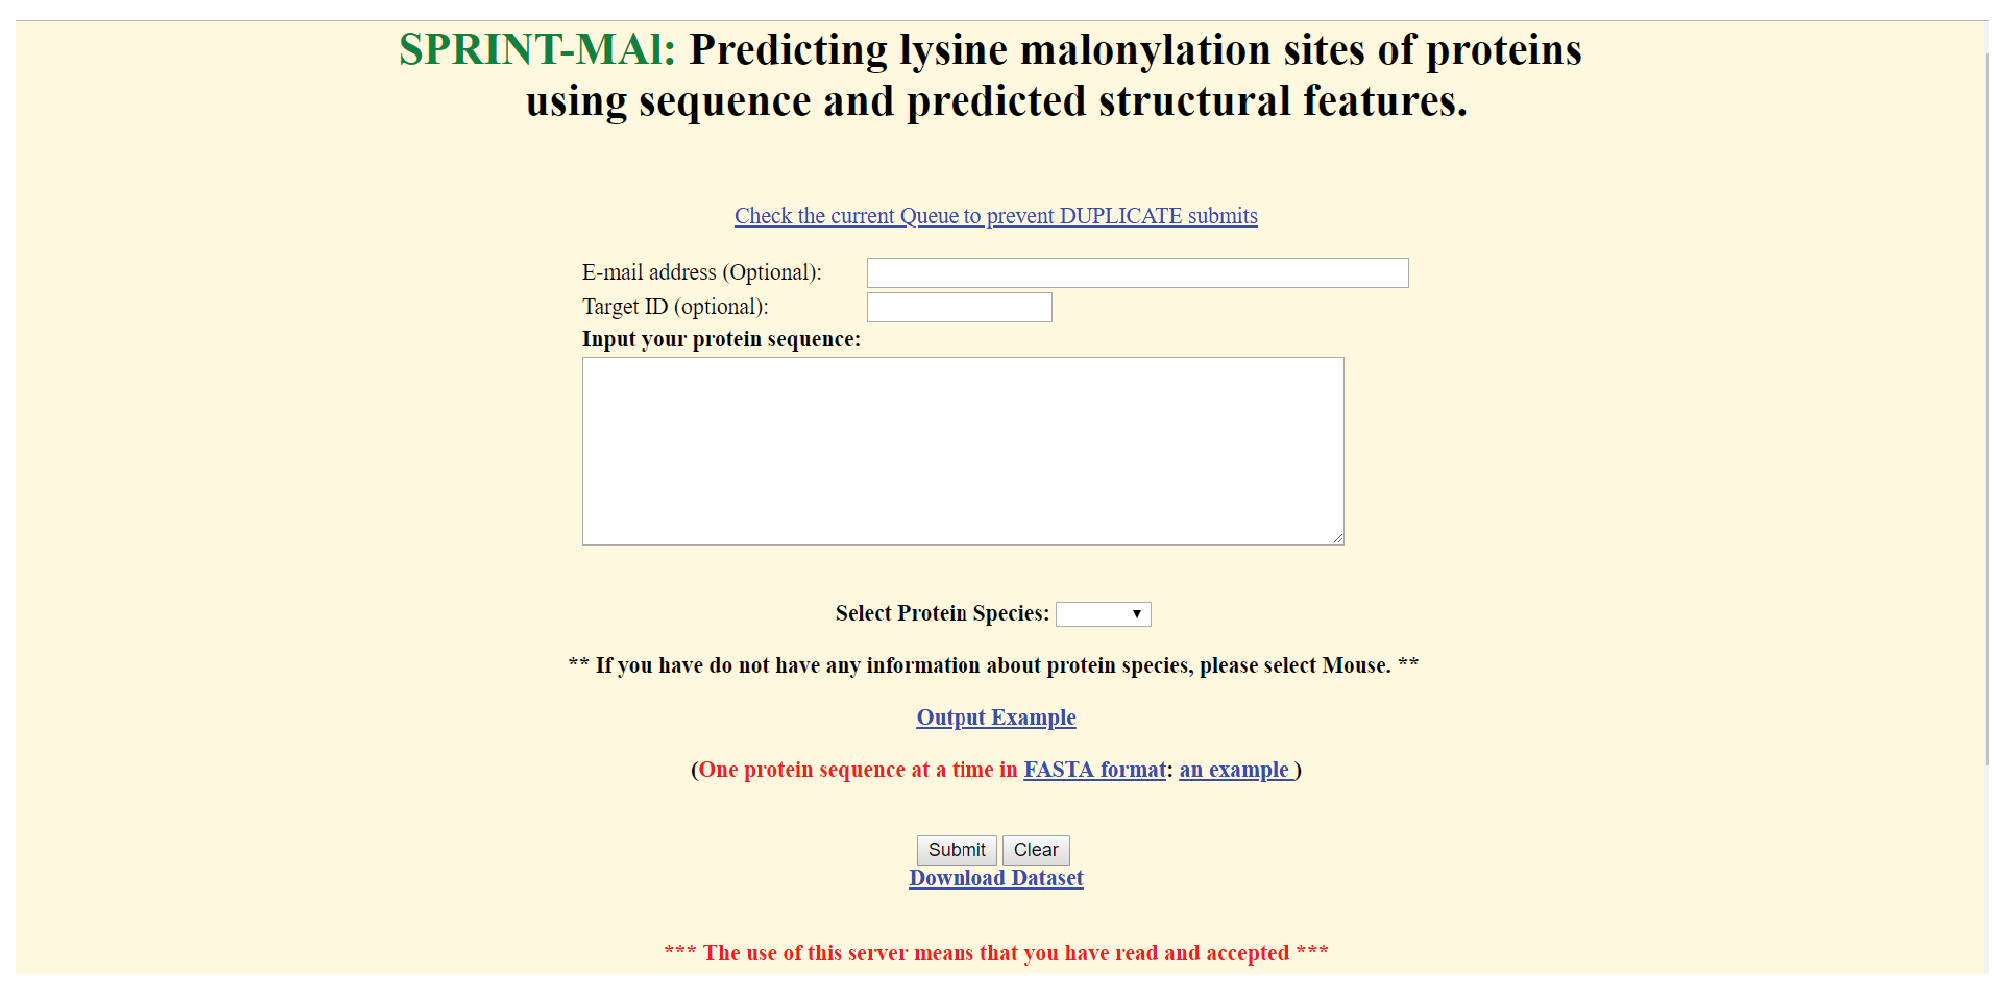
\includegraphics[width=\textwidth]{spintmal.eps}
    \caption{SPRINT-Mal}\centering \cite{Anderson04}
  \end{minipage}
  \hfill
  \begin{minipage}[b]{0.4\textwidth}
    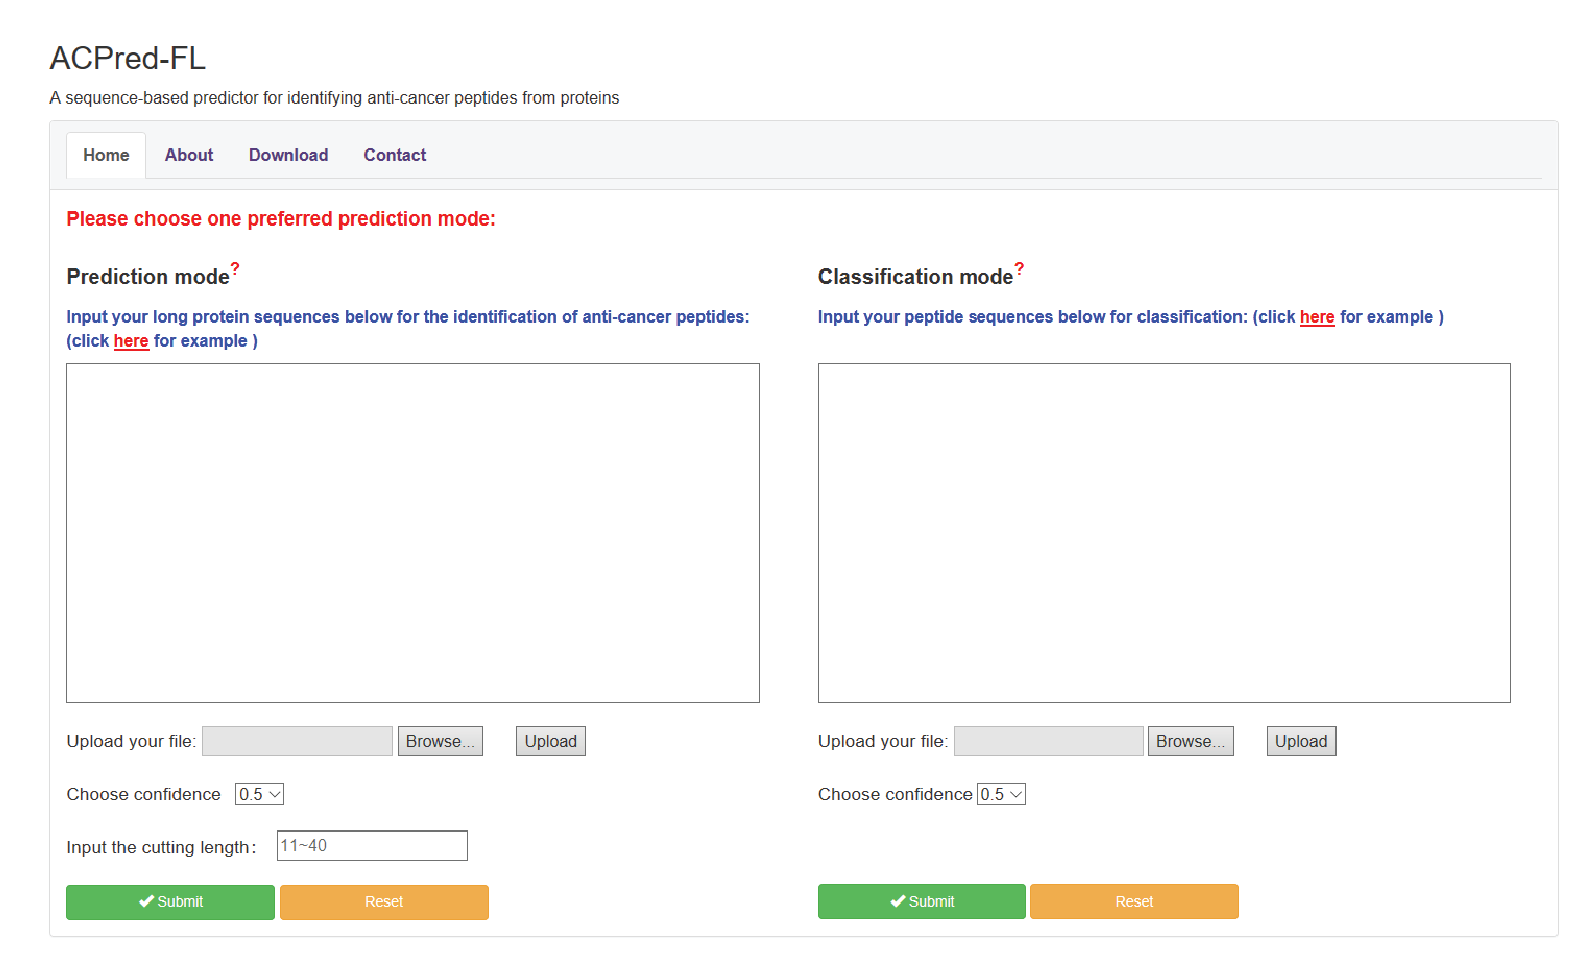
\includegraphics[width=\textwidth]{Anticancer.eps}
    \caption{ACPred-FL} \centering \cite{Anderson05}
  \end{minipage}
\end{figure}

\section{Comparison of Recent Workable Tools}
We have found some difference, when we studied the tools. Some comparison between the tools are given below :
\begin{table}[htbp]
\caption[Comparison of Recent Workable Tools]{Sprint-Mal \& ACPred-FL }
\centering
\footnotesize
\resizebox{\textwidth}{!}{\begin{tabular}{|c| >{\centering\arraybackslash}p{4.5cm} | >{\centering\arraybackslash}p{4.5cm} |} \hline
\bf No. & \bf Sprint-Mal & \bf ACPred-FL \\\hline
1. & There is option to input as mail for tracking user & There is option to take any input for tracking user  \\\hline
2. & There are some rule and regulation & There is no rule and regulation \\\hline
3. & It works on two data set so there is a choice option of prediction & It works only one data set so there is no option \\\hline
4. & There is only one option of prediction & There is two option for Identification and prediction  \\\hline
5. & There is no option to set up confidence level & There is option of choose confidence level  \\\hline

\end{tabular}}
%\label{training_testing_examples_KDD99}
\end{table}

\section{Software Requirement Specification (SRS)}
This document lays out a project plan for the development of "A tool for Prediction of Anticancer Peptide Using Sub spacing Ensemble Classifier". The plan will include, but is not restricted to a summary of the system functionality, the scope of the project from the perspective of the "Anticancer Prediction Problem" team (me, my team members and my supervisor), scheduling and delivery estimates, project risks and how those risks will be mitigated, the process by which we will develop the project will be recorded throughout the project.
\subsection{Overview}
Anticancer Peptide Prediction using laboratory method is time consuming and expensive. With laboratory method prediction is fully dependent on laboratorians and financial capabilities of individuals. We aim to develop an application that would enable them to save their valuable time and money with nearly perfect prediction system.
\subsection{Purpose}
The purpose of SRS document is to present a detailed description of constraint of anticancer prediction. It will explain the purpose and features of our system used here and how the system will work, what type of algorithms will be used here and how this system will be operated. This document is intended for both stakeholders and developers of the system.
\subsection{Scope}
In our system anticancer peptides prediction can be hazard free and cheap. Biologists spends their valuable time and laboratory resources for the prediction of anticancer peptides. Those methods are highly expensive. Our system will help them to predict anticancer peptides absolutely free. Thus will help them to invent cure for cancer patients.
\subsection{Goals}
After the completion of this project we aspire to fulfill some specific goals. Some of the goals are listed below. 
\begin{itemize}
\item Predict anticancer peptide using our developed tool
\item Help biologists/clinical researcher in the field of finding cancer cure
\item Reducing the cost of anticancer peptide prediction
\item Help saving time of researchers/biologists
\end{itemize}
\subsection{Overall Description}
Here we have described the overall process elaborately to provide as much as information about our project we can in an organized way.
\subsubsection{Users}
There will be mainly two kind of users of our web tool who are Clinical Researcher and Biologists.
\subsubsection{Functionality}
It is important to understand how our web tool will function. Down below we have listed the functionality of our web tool.
\begin{itemize}
\item User would be able to predict anticancer peptides 
\item User will provide protein sequence and our tool will predict attribute according to that
\item After prediction, predicted result will be shown to the user as a response message.
\end{itemize}
\subsubsection{Platform}
Our project will be launched as a Web-based application which will be accessed by a web browser which has an internet connection.
\subsubsection{Development and Responsibility}
We would be developing the software and we are responsible for the creation of related interfaces, server connections and support.
\subsubsection{Functional Requirements}
The functional requirement is describing the behavior of the system as it relates to the system's functionality. A finely designed system's usability is always satisfactory. This anticancer peptides prediction systems portal and each of its pages are very much easy to use. User will find it comfortable and some good set of directives are given to guide the user doing different set of activities. The category of user interfaces depends on the privileges given to the users. All the basic user functions that the user can perform are shown at the homepage and they are just one click away to access those functions. Making it user friendly is one of our prime goals and there will be a feedback screen for the user if there are any issues to address.

\paragraph{Step-By-Step Description:}
Clinical researchers or biologists uses the web tool to predict anticancer peptides. 
\begin{figure}[H]
\centering
 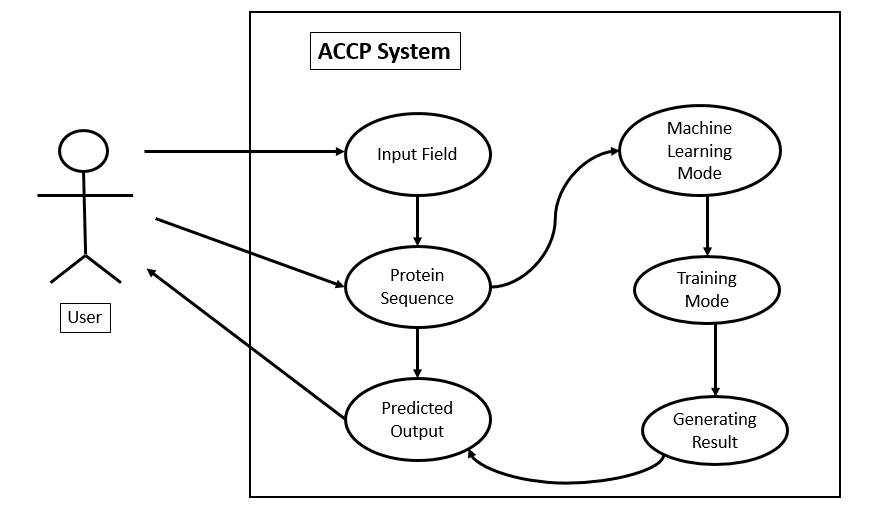
\includegraphics[width=0.7\textwidth]{useCase.PNG}
 \caption{Use Case Diagram of SRS}
 \label{fig:useCase}
\end{figure}
Use case diagram \ref{fig:useCase} also given which help us to visualize the whole process.
\begin{itemize}
\item Researchers/Biologists/User inserts protein sequence in the text field
\item That sequence is sent to the machine learning algorithm
\item Machine learning algorithm predicts anticancer peptide based on previously saved trained model
\item Prediction result is show to the user/researchers/biologists after predictions.
\end{itemize}

\subsubsection{Requirements Specification}
Let us discuss the non-functional requirements of our routine management system.
\paragraph{System Properties :}
The system properties are listed below which describes which tools were used to make this project and what are the requirements to run this tool.

\begin{description}
\item[(a)] A web based anticancer peptides prediction system runs on the internet
\item[(b)] Runs on Linux server
\item[(c)] HTML/CSS, Bootstrap, JavaScript based UI design
\item[(d)] Python flask based functioning system.
\end{description}
\paragraph{Storage Requirements :}
The storage requirements for the project are described down below.
\begin{description}
\item[(a)] Different contents uploaded to the system are preserved
\item[(b)] Minimum and maximum requirements of disk space are considered with care
\item[(c)] Unnecessary and obsolete contents are removed to free the disk space.
\end{description}
\paragraph{Accessibility :}
Here we have stated the means by which someone can access this web tool.
\begin{description}
\item[(a)] This system is accessible from mobile/desktop/laptop devices
\item[(b)] A stable internet connection is required.
\end{description}
\paragraph{Documentation :}
Proper documentations make it easier to use any system. We will provide visual directions and instructions to use this web tool.
\begin{description}
\item[(a)] User guidelines to use the system with screen-shots will be provided
\item[(b)] User privileges and access management guidelines will be added in the documentation.
\end{description}
\paragraph{Availability :}
The system will be available to its specific users as stated below.
\begin{description}
\item[(a)] Any user can access this system 24/7
\item[(b)] A minimum amount of downtime will be taken during maintenance period.
\end{description}
\subsubsection{Technical Process}
Following would be the languages we would like to use for the development of our application within the stipulated time period.
\paragraph{Front-end development :}
HTML, CSS, Bootstrap, JavaScript.
\paragraph{Back-end development :}
\begin{itemize}
\item Programming Language : Python
\item IDE : Anaconda, Notepad++, Spyder
\item Virtual Machine : Vagrant Box. 
\end{itemize}

\section{Summary}
In this chapter we know about existing works and SRS. Which inspired us and helped us to develop our project.  
\chapter{Machine Learning Methodology} \label{Methods}
\ifpdf
    \graphicspath{{chapter_3/figures/PNG/}{chapter_3/figures/PDF/}{chapter_3/figures/}}
\else
    \graphicspath{{chapter_3/figures/EPS/}{chapter_3/figures/}}
\fi
\section{Introduction}
This section provides the details of materials and methods used in this project. As suggested by K. C. Chou in \cite{chou2011some}, we have followed the famous five steps: i) selection of a proper dataset; ii) representation of peptides using feature extraction; iii) selection of a classification algorithm; iv) evaluation methodology and v) establishment of a web server as a prediction tool. In the testing phase, we generate a large number of features based on the peptide sequences taken from the dataset. After that, the feature space is divided into thee parts and each are learnt using a weak classifier. The majority voting technique is used to provide with the final prediction decision from the weak classifiers. The ensemble is saved for the testing phase and used to predict anticancer property for any unknown peptide sequence. Rest of this section delineates the steps followed in this work.

\section{Benchmark Dataset}
In this project, we have used the training dataset constructed and presented by Wei et al. in \cite{wei2018acpred}. One major problem in the previous datasets prior to this work was the imbalance with the negative instances. This newly proposed dataset was based on previously available databases of ACPs \cite{tyagi2013silico,tyagi2014cancerppd,chen2016iacp}. Among all the available ACPs, CD-HIT \cite{li2006cd} was used to remove instances with 90\% or more similarity. From that 250 positive and 250 negative samples were selected to construct the training dataset. Table~\ref{tab:dataset} provides a summary pdf the dataset. Formally, the dataset $\mathbb{S}$ can be shown as below: 
$$\mathbb{S}=\mathbb{S}^+ \cup \mathbb{S}^-$$
Here, $\mathbb{S}^+$ and $\mathbb{S}^-$is the set of positive and negative instances respectively.
\begin{table}[h]
\centering
\begin{tabular}{c|c|c}
    \bf Type &\bf  Number of Instances &\bf Label  \\
    \hline 
    Anticancer Peptide & 250 & +1\\
    Non Anticancer Peptide & 250 & -1\\
    \hline
    Total & 500\\
\end{tabular}
\caption{Summary of the dataset. \label{tab:dataset}}
\end{table}


\section{Feature Collection}
After selection of the dataset, now we have to choose a proper way to represent each peptide $P\in \mathbb{S}$. Each peptide instance in the dataset is replaced by a set of features and thus converted into a feature vector formally shown as below:
$$P=[ f_1 f_2 f_3 \cdots f_n]$$

Note that, here each peptide sequences $P \in \mathbb{S}$ is a small string of amino-acids from the alphabet, $\Sigma$ that contains 20 different symbols. Here, $f_i$ is a feature extracted from the peptide instance. In this project, we generate different sequence based features that are easy to generate and also follows the common view that information flows from the genetic code and must be hidden in the peptide sequence itself. We provide a brief description of the features generated for our work

\begin{figure}[H]
\centering
 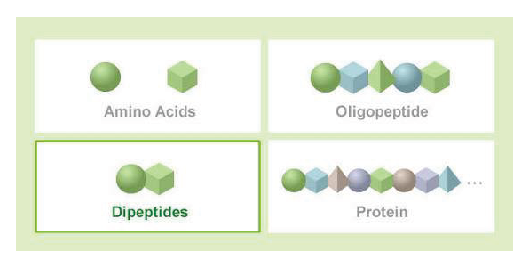
\includegraphics[width=0.5\textwidth]{f1.eps}
 \caption{Feature Collection}\cite{Anderson06}
\end{figure}

\subsection{Monomer Composition}
Monomer composition is simply the normalized frequency of the count of different amino acid monomers in the given peptide sequence. Since there are only 20 different amino acids, the number of features is 20. Here monomer composition is represented by $f_1$.

\begin{figure}[h]
\centering
 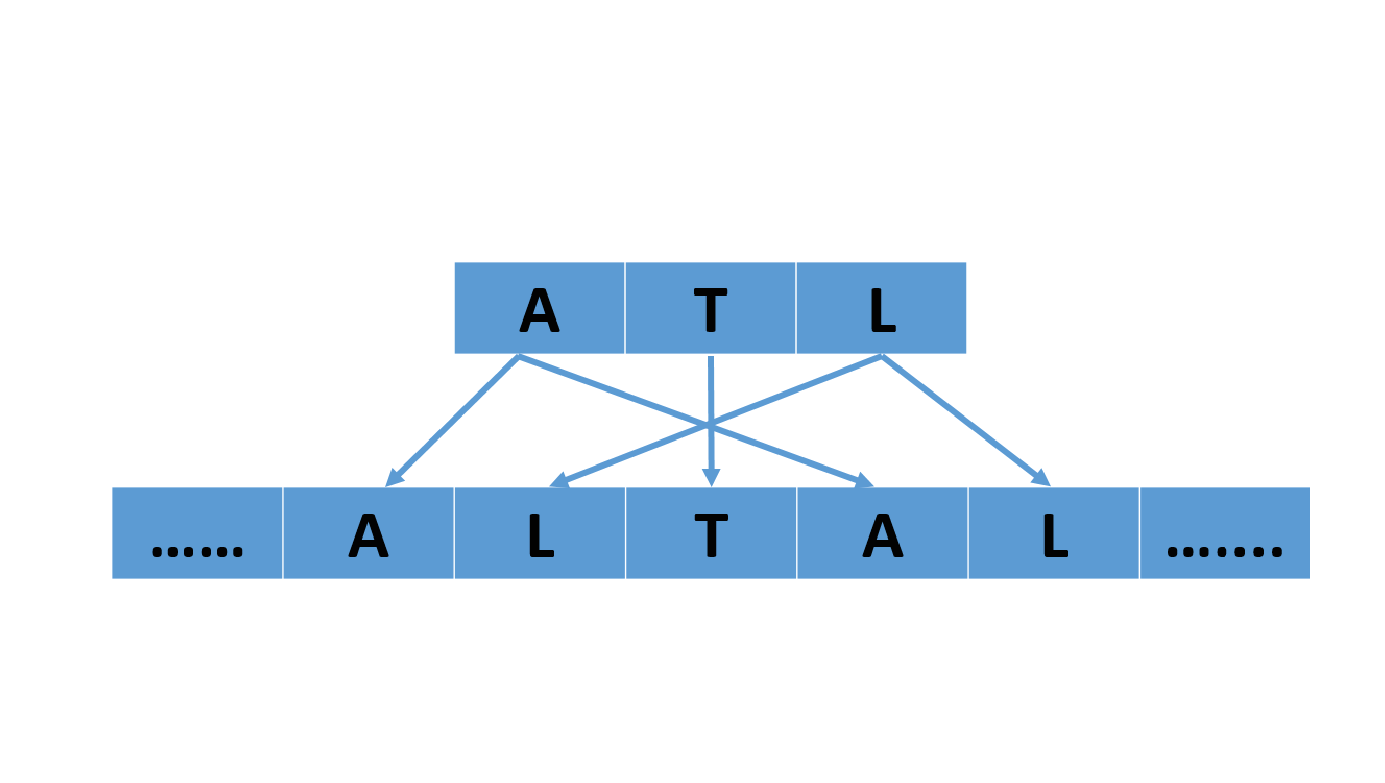
\includegraphics[width=0.7\textwidth]{mononew.eps}
 \caption{Monopeptide Composition}
\end{figure}

\subsection{Dipeptide Composition}
Dipeptide composition is the normalized frequency of the different dipeptides. Dipeptides are of 400 types and so is the number of features generated. Here monomer composition is represented by $f_2$.
    
\begin{figure}[H]
\centering
 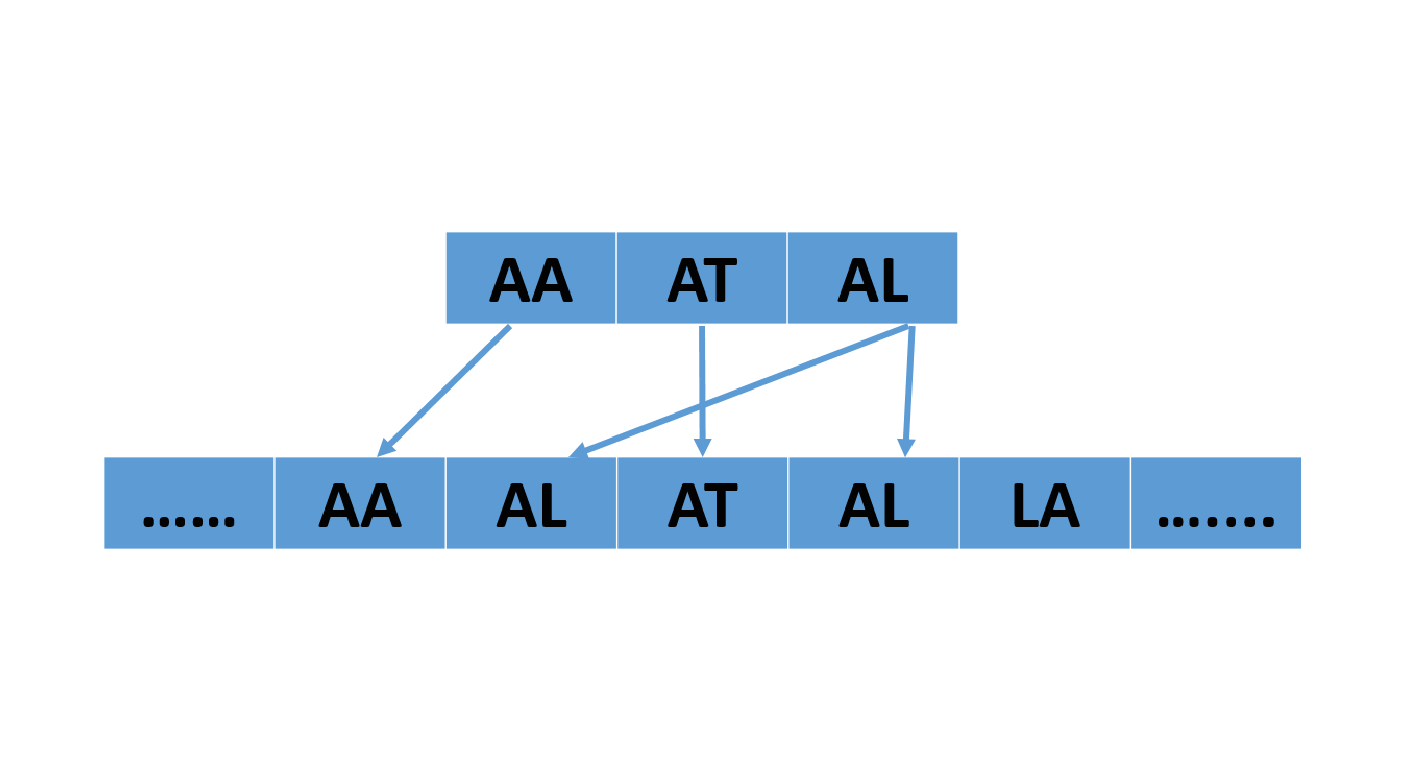
\includegraphics[width=0.7\textwidth]{Dipeptidenew.eps}
 %\caption*{\scriptsize Source:\url{https://www.kyowa.eu/products/new-products/dipeptides.html}}
 \caption{Dipeptide Composition}
\end{figure}

\subsection{Tripeptide Composition}
We have also considered tripeptide composition which is the normalized frequency of tripeptides. The total number of tripeptides are 8000. Here monomer composition is represented by $f_3$.

\begin{figure}[H]
\centering
 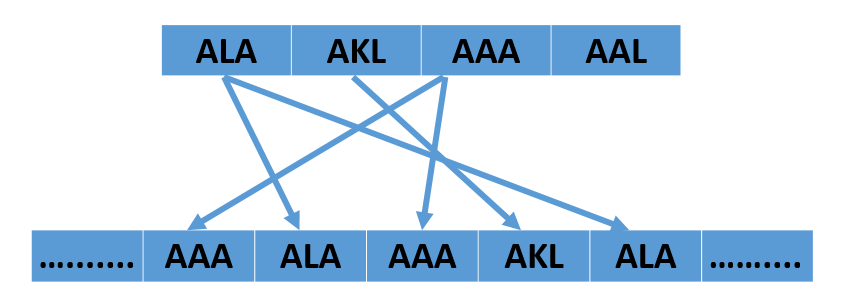
\includegraphics[width=0.7\textwidth]{tripeptide.PNG}
 %\caption*{\scriptsize Source:\url{https://www.kyowa.eu/products/new-products/dipeptides.html}}
 \caption{Tripeptide Composition}
\end{figure}

\subsection{1-gapped Di-mono Composition}
We have also considered the normalized frequency of tripeptides with a single gap in them. The particular patterns are in the form of $XX\_X$. The number of features are 8000.

\begin{figure}[H]
\centering
 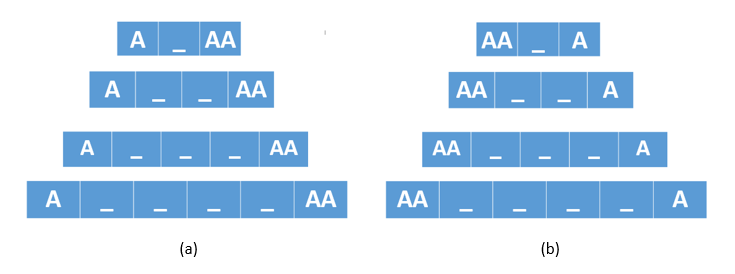
\includegraphics[width=0.7\textwidth]{comGap.PNG}
 %\caption*{\scriptsize Source:\url{https://www.kyowa.eu/products/new-products/dipeptides.html}}
 \caption{(a) 1-gapped Mono-Di Composition and (b) 1-gapped Di-mono Composition}
\end{figure}

\subsection{1-gapped Mono-Di Composition}
Similarly we have also considered normalized frequency of tripeptides with a single gap in them in the form of $X\_XX$. The number of features are 8000.

\subsection{Feature Collection Summary}
We have divided the generated features into three non-overlapping groups. Summary of the features and subspacing are given in Table~\ref{tab:features}.

\begin{table}[h]
    \centering
    \begin{tabular}{c| c| c| r}
        Feature Subspace & Features & Type & Number of features \\
        \hline
        $G_1$ & $f_1$ & Monomer Composition & 20\\
        & $f_2$& Dipeptide Composition & 400\\
        & $f_3$& Tripeptide Composition & 8000\\
        \hline 
        $G_2$ & $f_4$ & 1-gapped Di-mono Composition & 8000\\
        \hline 
        $G_3$ & $f_5$ & 1-gapped Mono-Di Composition & 8000\\
    \end{tabular}
    \caption{Summary of features and feature subspacing.    \label{tab:features}}

\end{table}

\section{Classification Algorithm}
We have used a feature subspacing based ensemble classification algorithm as a classifier in this work. Fig.~\ref{fig:en} shows a block diagram for the classifier used. After the feature extraction phase, the total number of feature are divided into three groups as shown in the figure and also in Table~\ref{tab:features}. Each of these feature vectors are then zipped with the peptide labels to train individual classifiers. Since there are three parts, we will need three different classifiers for training.  
\begin{figure}[h]
    \centering
    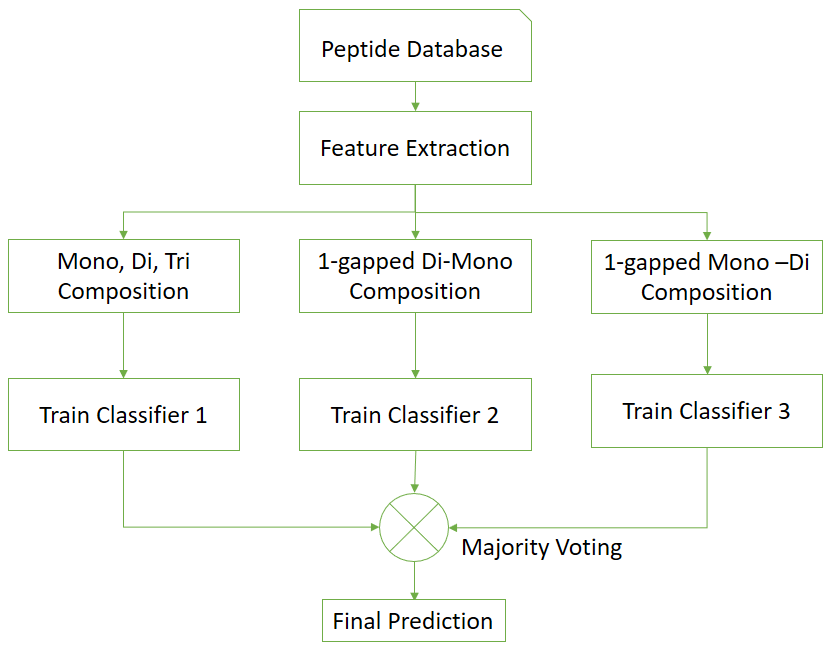
\includegraphics[width=0.8\textwidth]{ensemble}
    \caption{Block diagram of the feature subspacing ensemble classifier.     \label{fig:en}}
\end{figure}

Note that three single classifiers used to train three subspaces of the feature space are not required to be of the same type. After the training each will learn their own model and predictions from each of these single classifiers will be aggregated using a simple majority voting for the final prediction. In the testing phase three models are to be saved in order to be used along with the voting scheme. Note that, we have not utilized any weighted voting here. Also the choice of dividing the feature space into three parts was also done arbitrarily. Weighted schemes, overlapped feature subspacing and number of subspaces could be left for future exploration. 

\section{Used Algorithm}
We used K nearest neighbor\cite{Anderson07}, naive bayesian\cite{Anderson08}\cite{Anderson09}, support vector machine\cite{Anderson10}, decision tree\cite{safavian1991survey} and logistic regression\cite{hosmer2013applied} for predicting the result.

\section{Parameter of Using Algorithms}
The table shows the parameter of algorithms.
\begin{table}[htbp]
\caption[Parameter of Algorithm]{Parameter of Algorithm }
\centering
\footnotesize
\resizebox{\textwidth}{!}{\begin{tabular}{|c| >{\centering\arraybackslash}p{3.5cm} |c|} \hline
\bf Classifier & \bf Parameters & \bf Types \\\hline
K-Nearest Neighbor & Number of Neighbors, Training set, test instances and defaults & -  \\\hline
Naïve Bayes & Training set, test instances and defaults & Bernoulli \\\hline
Support Vector Machine & Training set, test instances and defaults & Support Vector Classifier \\\hline
Decision Tree & Training set, test instances and defaults & - \\\hline
Logistic Regression & Training set, test instances and defaults & -  \\\hline

\end{tabular}}
%\label{training_testing_examples_KDD99}
\end{table}

\section{Performance Evaluation}
In the literature of supervised learning methods for any prediction task, it is shown that selection of performance evaluation methods in very important \cite{chou2011some}. For the sake of comparison, we have used the standard set of metrics and evaluation methods for the performance evaluation of our method as well. We have used 10-fold cross validation technique for the sampling on the train set. Here, the train set is divided into 10 folds or parts shuffled randomly and each time, a single fold in used as testing while the rest of the dataset is used for training. 

We have used eight standard metrics for as performance measure: Accuracy (Acc), Sensitivity (Sn), Specificity (Spc), Precision, Recall, F1-Score, Matthew's Correlation Coefficient (MCC) and area under Receiver Operating Characteristic curve (auROC). For any binary classification task, we assume $TP$ be the number of true positives or number of correctly predicted positive instances and $TN$ be the number of true negatives or number of correctly predicted negative instances. Let FP and FN denote number of false positive and false negatives. They are respectively negative instances incorrectly predicted as positive and  positive instances incorrectly predicted as negative. Now the metrics are defined as in below:    

\small{
\[ Acc = \frac{TP + TN}{TP + FP + FN + TN} \times 100\% \]
\[ Sn = \frac{TP}{TP + FN} \times 100\% \]
\[ Spc = \frac{TN}{TN + FP} \times 100\% \]
\[ Precision = \frac{TP}{TP + FP} \]
\[ Recall = \frac{TP}{TP + FN}\]
\[ F1-Score = \frac{2 \times precision \times recall}{precision + recall}\]
\scriptsize{
\[ MCC = \frac{(TP \times TN) - (FN \times FP)}{\sqrt{(TP+FN) \times (TN+FP) \times (TP+FP) \times (TN+FN)}} \]
}}

We have also considered auROC or area under Receiver Operating Characteristic (ROC) curve. ROC curve is the plot of TPR against FPR for different thresholds from a probabilistic classifier. Here note that each of this measures have the values in the range [0,1] except MCC. Here 0 means a worst classifier and 1 means a perfect classifier. In the case of MCC the values are in the range of [-1,+1]. 

\section{Summary}

In this chapter we have discussed about our collected features, our used algorithms.


	
\chapter{Experimental Results and Discussion} \label{Result}

\ifpdf
    \graphicspath{{chapter_5/figures/PNG/}{chapter_5/figures/PDF/}{chapter_5/figures/}}
\else
    \graphicspath{{chapter_5/figures/EPS/}{chapter_5/figures/}}
\fi

\section{Introduction}
In this section, we present the experimental results and analysis of our method. All the experiments were run five times and only the averages are reported as the classifiers used here are stochastic in nature. The classifiers were implemented using Scikit-learn library and Python 3.

\section{Result of used Algorithm}
The main goal of this work was to show that feature subspaced ensembles works better in comparison to the single classifiers. Without changing the feature subspacing as shown in the last section, we have use five different weak classifiers and their combinations in the ensemble. They are: Decision Tree (DT), Support Vector Machines (SVM), K-Nearest Neighbor (KNN), Logistic Regression (LR) and Naive Bayesian Classifier (NB). Note that we are performing 10-fold cross validation. Firstly, in Table~\ref{tabSingle}, we present the results achieved by each of these single classifiers on the dataset. Here, we note that performance of all the classifiers are similar. However, KNN performs little worse to other single classifiers. Note that the full set of features were fed to these single classifiers.




\begin{table}[h]
\centering
\begin{tabular}{l|p{1.5cm}p{1.2cm}p{1cm}p{1cm}p{1cm}p{1cm}p{1cm}p{1cm}} \hline
\bf Classifier & \bf Precision & \bf Recall & \bf F1 & \bf Acc & \bf MCC & \bf Sn& \bf Spc & %\bf TP & \bf FP & \bf FN  & \bf TN & 
\bf AuROC \\\hline
SVM & 0.8386 & 0.7152 & 0.7567 & 77.08 &  0.5686 & 80.61 & 74.41 & %207 & 71 & 43 & 179 & 
0.8528   \\\hline
NB & 0.6821 & 0.9440 & 0.7978 & 75.88 & 0.5614 & 68.84 & 91.32 & %143 & 13 & 107 & 237 & 
0.7588   \\\hline
KNN & 0.7431 & 0.3632 & 0.5007 & 64.50 & 0.3434 & 82.12 & 59.10 & %230 & 159 & 20 & 91 & 
0.7650   \\\hline
LR & 0.8605 & 0.7768 & 0.7869 & 78.92 & 0.5840 & 79.18 & 78.68 & %199 & 54 & 51 & 196 & 
0.8657  \\\hline
DT & 0.6760 & 0.7288 & 0.7302 & 73.36 & 0.4710 & 73.61 & 73.15 & %185 & 68 & 65 & 182 & 
0.7336  \\\hline
\end{tabular}
\caption{Performance of single classifiers on the dataset. \label{tabSingle}}
\end{table}



\begin{table}[h]
\centering
\begin{tabular}{l|p{1.5cm}p{1.2cm}p{1cm}p{1cm}p{1cm}p{1cm}p{1cm}p{1cm}} \hline
\bf Classifier & \bf Precision & \bf Recall & \bf F1 & \bf Acc& \bf MCC & \bf Sn& \bf Spc& %\bf True Positive & \bf False Positive & \bf False Negative  & \bf True Negative & 
\bf AuROC \\\hline
SVM+SVM+SVM & 0.9245 & 0.9512 & 0.8247 & 79.00& 0.6296 & 70.89& 97.24& %149 & 4 & 101 & 247 & 
0.9345   \\\hline
NB+NB+NB & 0.8234 & 0.9376 & 0.8234 & 79.80& 0.6230 & 73.29& 91.39 & %165 & 16 & 85 & 234 & 
0.8530   \\\hline
KNN+KNN+KNN & 0.9001 & 0.384 & 0.8151 & 78.64& 0.6036 & 71.94& 91.22& %159 & 15 & 91 & 235 & 
0.9166 \\\hline
LR+LR+LR & 0.8739 & 0.9220 & 0.8242 & 80.24 & 0.6083 & 74.35 & 89.96& %170 & 19 & 80 & 231 &
0.8969  \\\hline
DT+DT+DT & 0.8199 & 0.8288 & 0.8202 & 81.88& 0.6376 & 81.01 & 82.46 & %201 & 43 & 49 & 207 & 
0.8596  \\\hline
SVM+NB+LR & 0.8201 & 0.9736	& 0.7994 & 75.48& 0.5687 & 67.73 & 94.10 & %134 & 7 & 116 & 243 & 
0.8497 \\\hline
NB+LR+SVM & 0.8164 & 0.9736 & 0.7931 & 74.28& 0.5527 & 66.80 & 95.14 & %129 & 7 & 121 & 243 & 
0.8464 \\\hline
LR+SVM+NB & 0.8415 & 0.9776 & 0.8032 & 75.52 & 0.6539 & 67.81 & 95.99& %134 & 6 & 116 & 244 & 
0.8488 \\\hline
DT+SVM+DT & 0.7735 & 0.8944 & 0.8058 & 78.60 & 0.5912 & 73.49& 87.29 & %169 & 26 & 81 & 224 & 
0.8206 \\\hline
SVM+DT+DT & 0.7416 & 0.8928 & 0.8038 & 78.28 & 0.5854 & 73.18 & 87.04 & %168 & 27 & 82 & 223 & 
0.7616 \\\hline
LR+LR+DT &\ 0.8730 & 0.8816 &\bf  0.8360 & \bf 82.52&\bf  0.6603 & 79.51 & 86.52& %192 & 30 & 57 & 221 &
0.8819 \\\hline
SVM+LR+DT & 0.8186 & 0.9488 & 0.7969 & 77.48& 0.5882 & 70.39 & 92.13& %150 & 13 & 100 & 237 &
0.8379 \\\hline
SVM+NB+DT & 0.7530 & 0.9528 & 0.8098 & 77.44& 0.6087 & 70.23 & 92.66& %149 & 12 & 101 & 238 & 
0.7895 \\\hline
\end{tabular}
\caption{Performance of different ensemble classifiers on the dataset. \label{tabEnsemble}}
\end{table}

Next, we applied the ensemble classifier proposed in this project using each of these single classifiers member of the ensemble. The first five rows of Table~\ref{tabEnsemble} shows the experimental results. Note that, in each case accuracy and other measures were enhanced by the ensemble compared to the single classifier. The best performing ensemble was the decision tree ensemble.

We have also tried several mixtures of single classifiers in the ensemble. Eight different combinations of the five single classifiers were tried and the results are shown in the last eight rows of Table~\ref{tabEnsemble}. Here note that a combination of logistic regression and decision tree is the best performing ensemble combination among all in terms of F1, MCC and Accuracy. Thus we select this combination as the best ensemble for our method.

\subsection{Comparison with other methods}
We have also compared the performance of the best ensemble combination to that of the previous methods in the literature. We have used four other methods for the sake of comparison: AntiCP \cite{tyagi2013silico}, Hajisharifi's method \cite{hajisharifi2014predicting}, iACP \cite{chen2016iacp} and ACPred-FL \cite{wei2018acpred}. Note that, we have not run their predictors, rather reported the 10-fold cross validation results as presented in the work by Wei et al. \cite{wei2018acpred}. The results are shown in Table~\ref{tab:Compare}. 


\begin{table}[h]
    \centering
    \begin{tabular}{l| p{1.5cm} p{1.5cm}p{1.5cm}p{1.5cm}p{1.5cm}}
\hline
\bf Predictors	&\bf  Sn &\bf 	Spc &\bf  Acc &\bf MCC&\bf AuROC\\
\hline
AntiCP\_AAC&	67.2&	86.0&	76.6&	0.542&0.84\\%168	35	215	82
\hline
AntiCP\_DC&	73.6&	85.2&	79.4&	0.592	&0.87\\%184	37	213	66
\hline
Hajisharifi’s method&	68.0&	86.4&	77.2&	0.553&0.84\\%	170	34	216	80
\hline
iACP&	72.8&	86.0&	79.4&	0.593&0.86\\%	182	35	215	68
\hline
ACPred-FL& 	84.8&	98.0&	91.4&	0.835	&0.94\\%212	5	245	38
\hline
Our Method & 79.5 & 86.5 & 82.5 & 0.660 & 0.88\\
\hline
 \end{tabular}
    \caption{Performance comparison of different state-of-the-art predictors on the benchmark dataset. \label{tab:Compare}}

\end{table}

Note that, the performance of our method is superior to all other methods except ACPred-FL. Now, ACPred-FL have used a large number of features compared to ours and also did perform feature selection that could have enhanced their performance.

\section{Summary}
In this chapter we know about results by using many algorithms and also know about the comparison of that used algorithms.		
\chapter{Standards and Impacts} \label{Impact}
\ifpdf
    \graphicspath{{chapter_4/figures/PNG/}{chapter_4/figures/PDF/}{chapter_4/figures/}}
\else
    \graphicspath{{chapter_4/figures/EPS/}{chapter_4/figures/}}
\fi
%Write few lines about this chapter.

%\chapter{Impact}
%Write in details about the datasets that you used in this research work.%

%\begin{table}[htbp]
%\caption[Dataset]{Number of instances in dataset.}
%\centering
%\footnotesize
%\begin{tabular}{|c|c|c|} \hline
%\bf Attack Types & \bf Training Examples & \bf Testing Examples \\\hline
%Normal & 97278 & 60592 \\\hline
%Denial of Service & 391458 & 237594 \\\hline
%Remote to User & 1126 & 8606 \\\hline
%User to Root & 52 & 70 \\\hline
%%Probing & 4107 & 4166 \\\hline
%Total Examples & 494021 & 311028 \\\hline
%\end{tabular}
%\label{training_testing_examples_KDD99}
%\end{table}


\section{Impacts}

\subsection{Introduction}
This section is contain the details about the impacts on various section of our project. 

\subsection{Biological Impact}

This work has a large impact on economy. It increase of probability to find new cure, new formula can be generated from the attributes. It may help to find new \& unknown diseases and also may help to find reason of a diseases.

\subsection{Machine Learning}

By doing this work new features can be generated in machine learning. Also generated new machine learning algorithm, new methods for detection \& prediction and user friendliness.

\subsection{Social Impact}
Cancer is a disease which has no proper treatment. And available treatments doesn't always guarantees of full recovery due to the unavailability of proper cures/medicine. It is also expensive. Most of the people cannot bear the expense due to high expenses. Our developed tool may help biologist/clinical researchers to find cures. Which will help the cancer patients \& save lives. 

\subsection{Economic Impact}

This work has a large impact on economy. Cancer treatment is extremely costly and time consuming. As patient's needs to go through a lots of diagnosis. Our developed tool may help the biologist/clinical researcher to find a better cure which will helpful for treatment. Biologist spends lots of money and time for detecting anticancer peptide using laboratory method. Those laboratory methods are highly expensive which also causes cancer treatments being expensive. But our system will be fully free and thus will help clinical researchers/biologists detect anticancer peptides with absolutely less amount.

\subsection{Ethical Impact}
Anti Cancer peptide dataset is open to all for use, so we can use the datasets without needing any permission. For codding we are using Anaconda cloud, which is a free software and using spider and jupiter IDE which is also free. For documentation latex is being used. It is also a free software. All software's are free.

\section{Standard}

\subsection{Introduction}
Every project should maintain some standards. We are developing our project by following some standards in coding, UI, web development, ethics and software process.
\subsection{Standards}
 %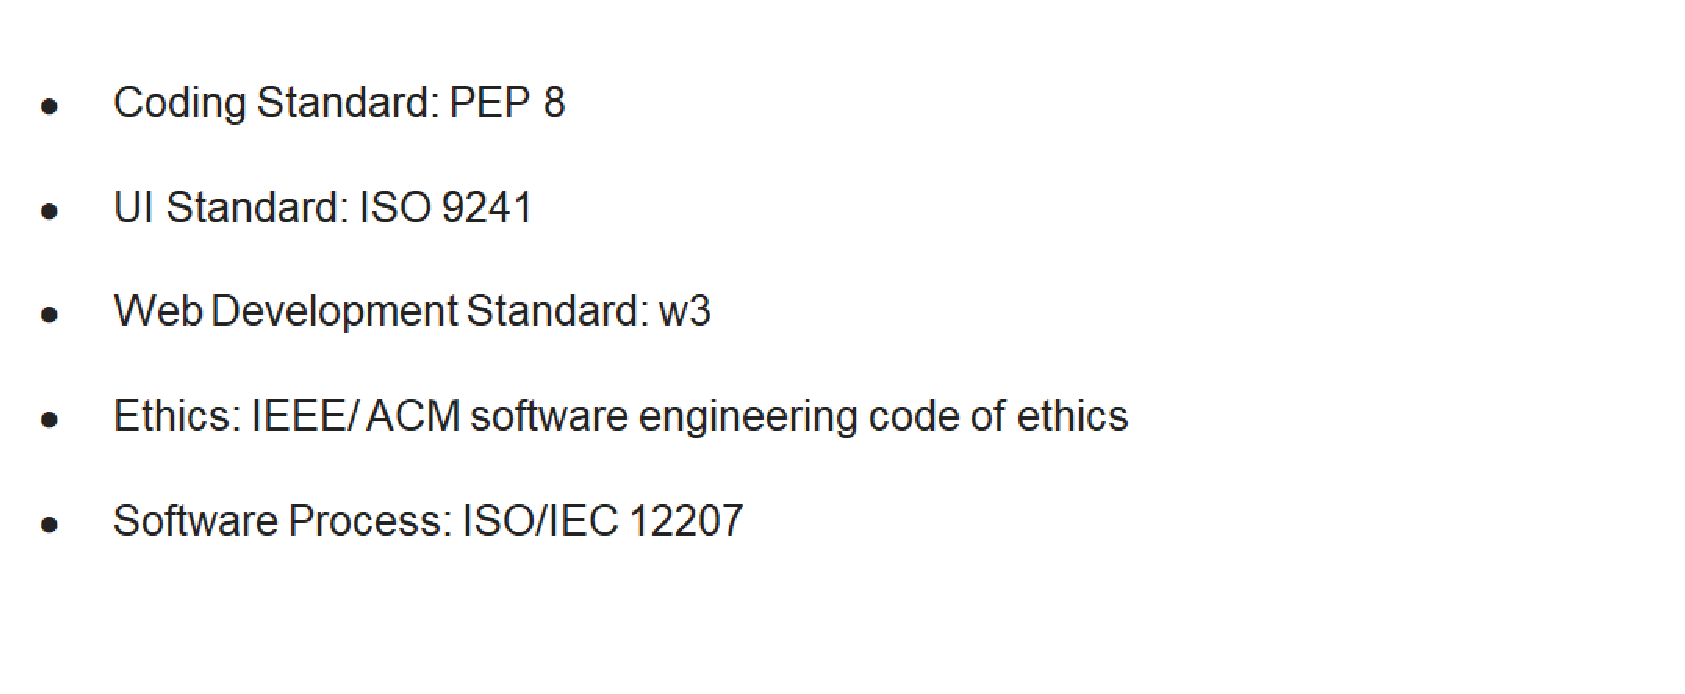
\includegraphics[width=\textwidth]{standard.eps}
 
\begin{description}[font=$\bullet$~\normalfont\scshape\color{red!50!black}]

\item Coding Standard: PEP 8
\item UI Standard: ISO 9241
\item Web Development Standard: w3
\item Ethics: IEEE/ ACM software engineering code of ethics
\item Software Process: ISO/IEC 12207

%\item [Coding Standard: ] PEP 8
%\item [UI Standard: ] ISO 9241
%\item [Web Development Standard: ] w3
%\item [Ethics: ] IEEE/ ACM software engineering code of ethics
%\item [Software Process: ] ISO/IEC 12207
\end{description}
 
As we are working on python so we have used PEP 8. ISO 9241 which is an international standard for UI, many country take it as their national standard so we took it as our UI standard. For web development we followed w3 because it is well organized platform. In ethical standard we have followed IEEE/ACM as they maintain professional standard. And lastly in software process we followed ISO/IEC 12207 because it gives us a common framework on the process of software life cycle.

\section{Challenges}

We have developed our tool using python for machine learning algorithm python flask package as API for parsing data from the input field to the machine learning algorithm. And we have also used HTML and CSS for the front end of the tool. The developed system is little bit different from other systems available right now. The system can't be run like other web tools just by coping the data on the server and hitting the web route. To run this system Linux server is must which allows installation of 3rd party application on which the system relies on. Linux server allows root level bash scripting which enables us to install dependencies for the system. But the issue with Linux server is it's not chip. But our university has helped us by providing us with a Linux server which helped us overcome the financial issue on buying a Linux server.\\
To be a capstone project every project needs to solve some complex issue. We think previous problem was one of them. And we have solved that problem with the help of our university authority. So this satisfies the condition of a project being a capstone project.

\section{Summary}

In this chapter we know about our projects social, biological, machine learning, economic, ethical impacts and constraint of our project and standards which we are following.


	
\chapter{Web Application} \label{Application}

\ifpdf
    \graphicspath{{chapter_7/figures/PNG/}{chapter_7/figures/PDF/}{chapter_7/figures/}}
\else
    \graphicspath{{chapter_7/figures/EPS/}{chapter_7/figures/}}
\fi

\section{Development}

The tool has been developed using flask framework. Flask is a framework of python. With this framework we have used some method of flask like Send, Post, Request and bash scripting. When user submit protein sequence on the input filed flask request helper passes that data to the controller. And using that controller the data is sent to the machine learning algorithm with the help of Post method. After the machine learning processes that data the predicted result is sent to the view/web page with the help of Send method.

\section{User manual}

Visit \url{http://fseacp.pythonanywhere.com} for the home page. After visiting the home page there will be menu buttons for different pages. To detect anticancer peptides go to \url{http://fseacp.pythonanywhere.com/server}. Insert your anticancer peptide sequence you want to predict in the text area as fasta format. After inserting your anticancer peptide sequence you can press clear button to clear out the text area or you can click submit button to check results. After clicking the submit button the input data will be passed to machine learning algorithm using controller and after processing the data then a post method will be sent to the server page with predicted result. If anticancer peptides are detected it send accuracy, "Anti-Cancer Peptide Detected" if not then "No Anticancer Peptides are Detected". If you enter a random string that doesn't match to an anticancer peptide the send response will be "Invalid Sequence". Here we also add some screen-shots. To see the contributors who worked for this tool click on the contributors menu button on the top right corner. To download datasets you can go to \url{http://fseacp.pythonanywhere.com/downloads}. Here we also add read me section \url{http://fseacp.pythonanywhere.com/readme} to make our website more user friendly.
\begin{figure}[H]
\centering
 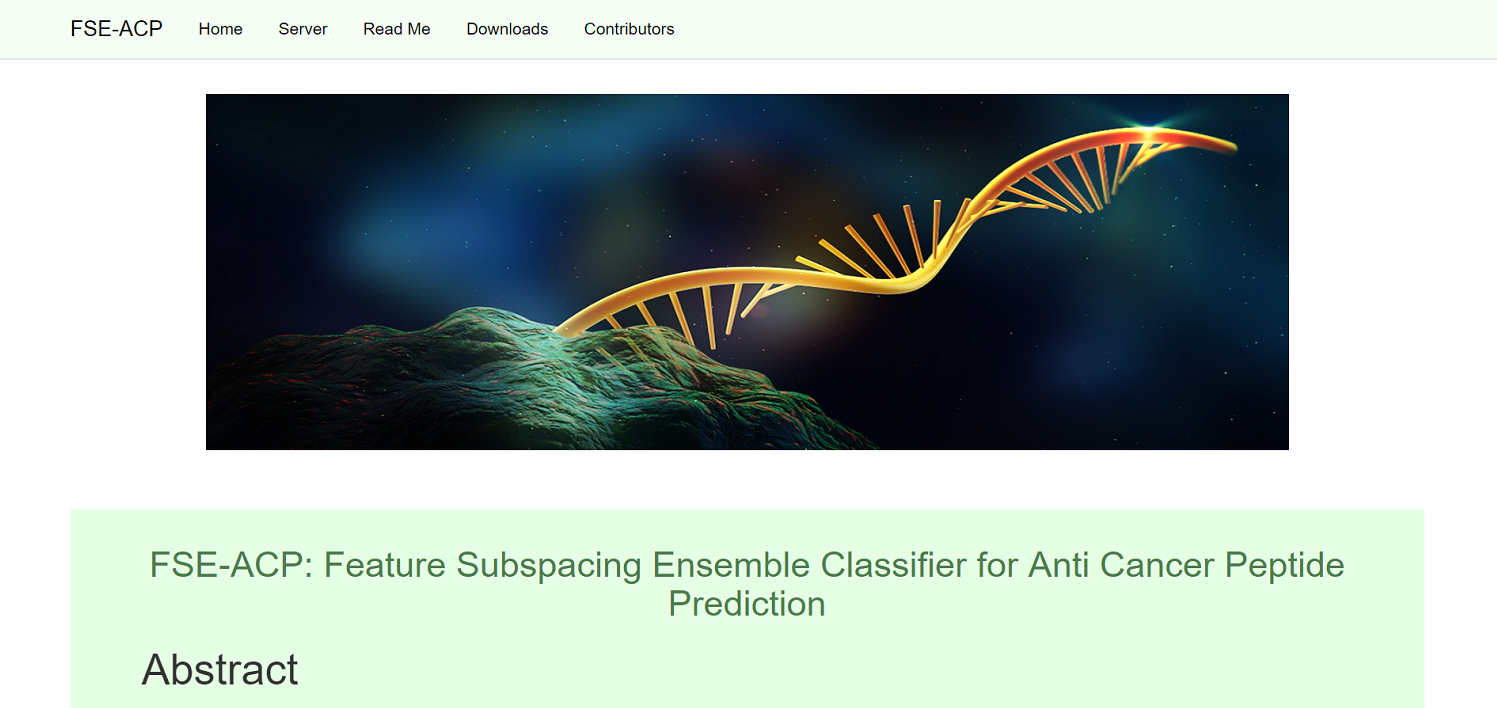
\includegraphics[width=0.8\textwidth]{home.png}
 \caption{Home Page}
\end{figure}
\begin{figure}[H]
\centering
 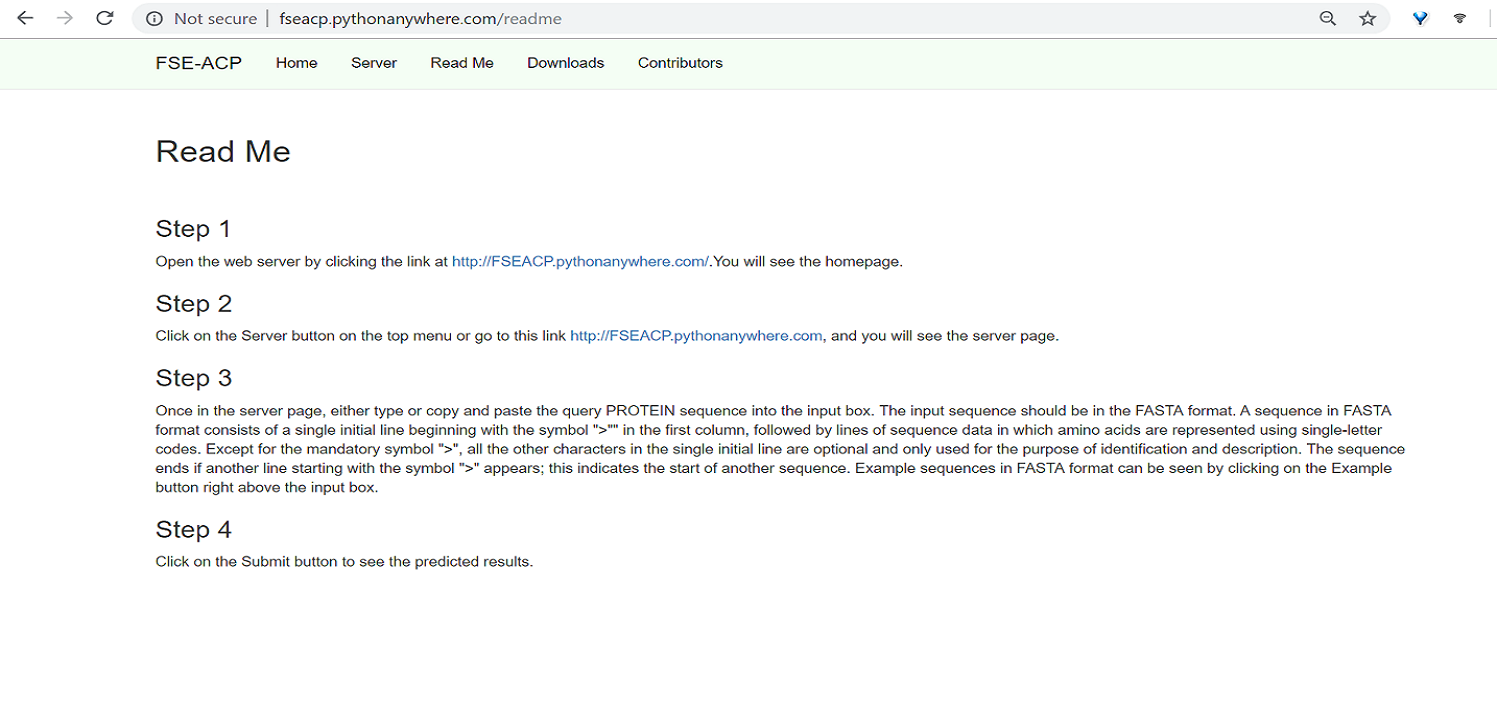
\includegraphics[width=0.8\textwidth]{read.png}
 \caption{Read Me Page}
\end{figure}
\begin{figure}[H]
\centering
 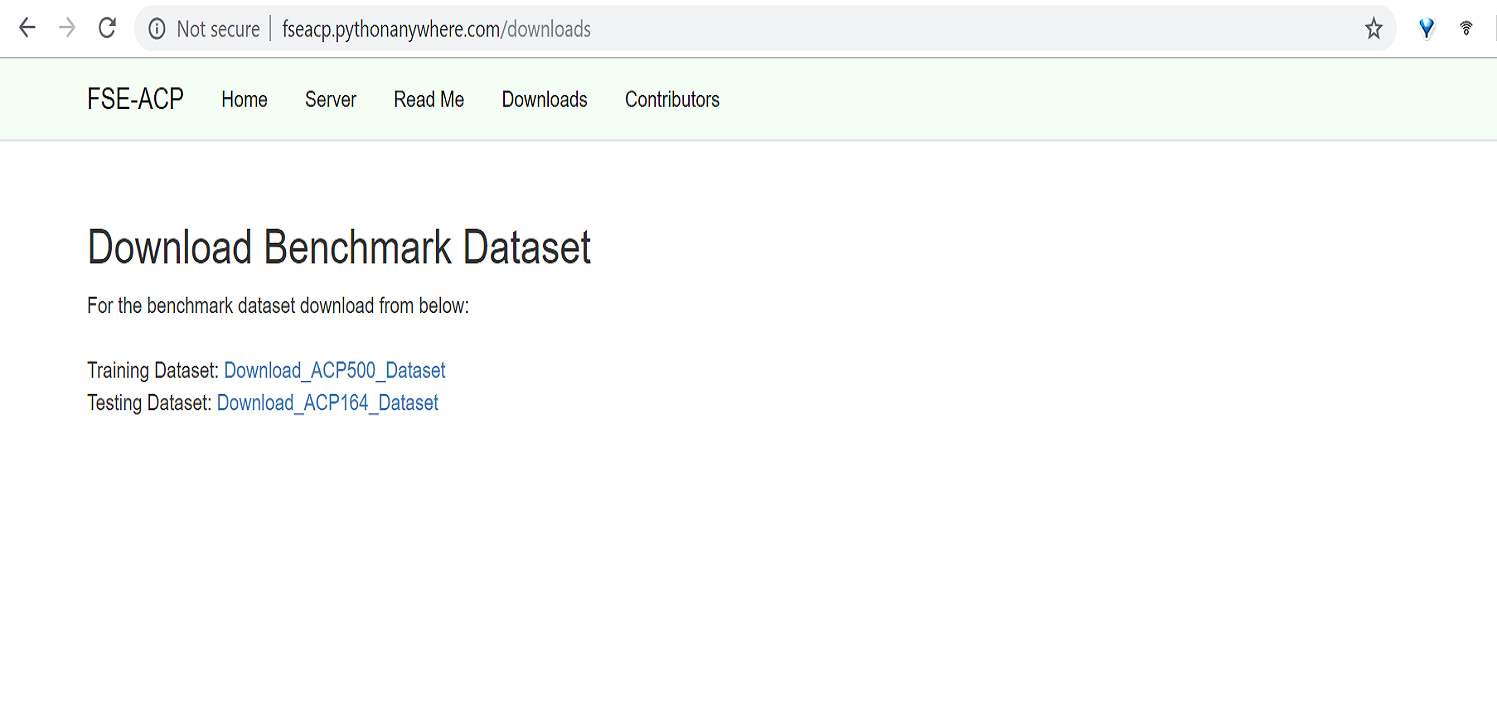
\includegraphics[width=0.8\textwidth]{dataset.png}
 \caption{Downloads Page}
\end{figure}
\begin{figure}[H]
\centering
 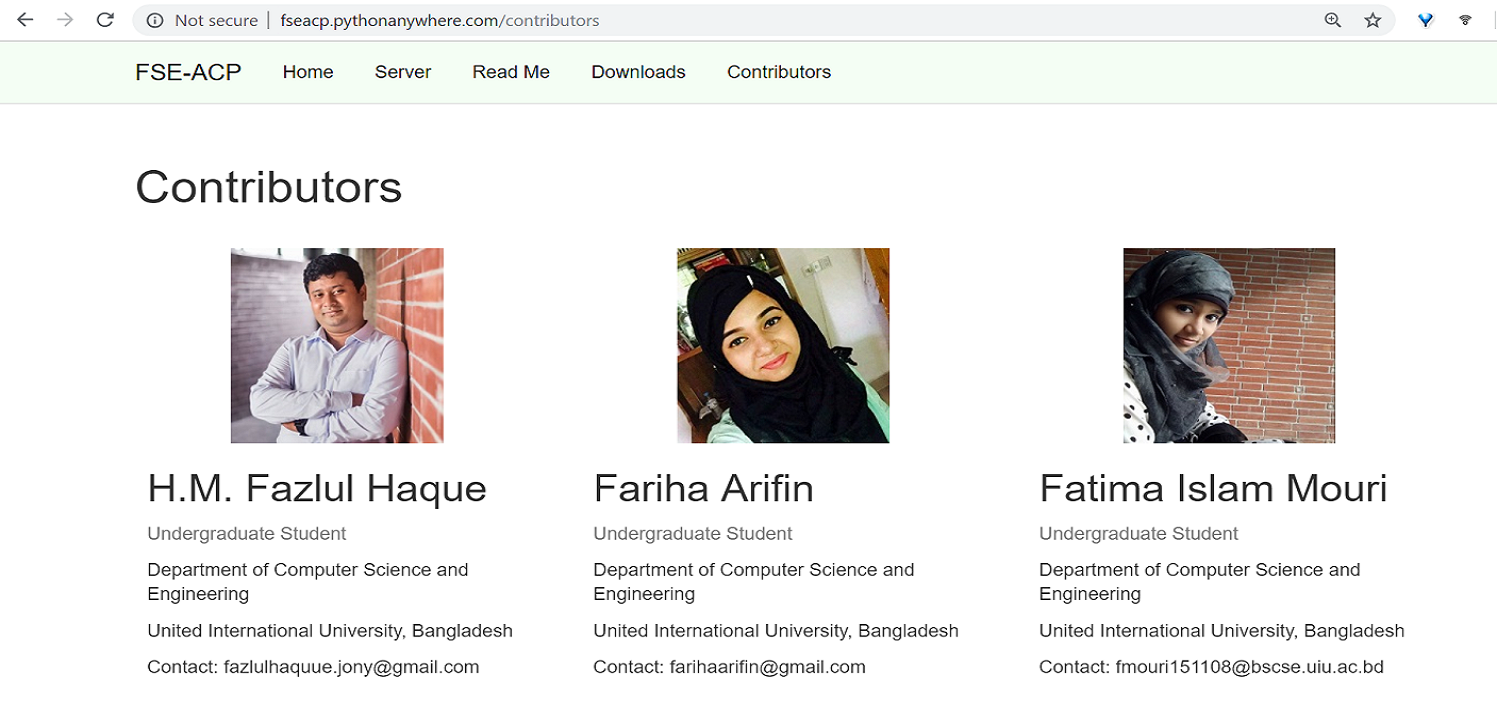
\includegraphics[width=0.8\textwidth]{contri1.png}
 \caption{Contributors Page}
\end{figure}
\begin{figure}[H]
\centering
 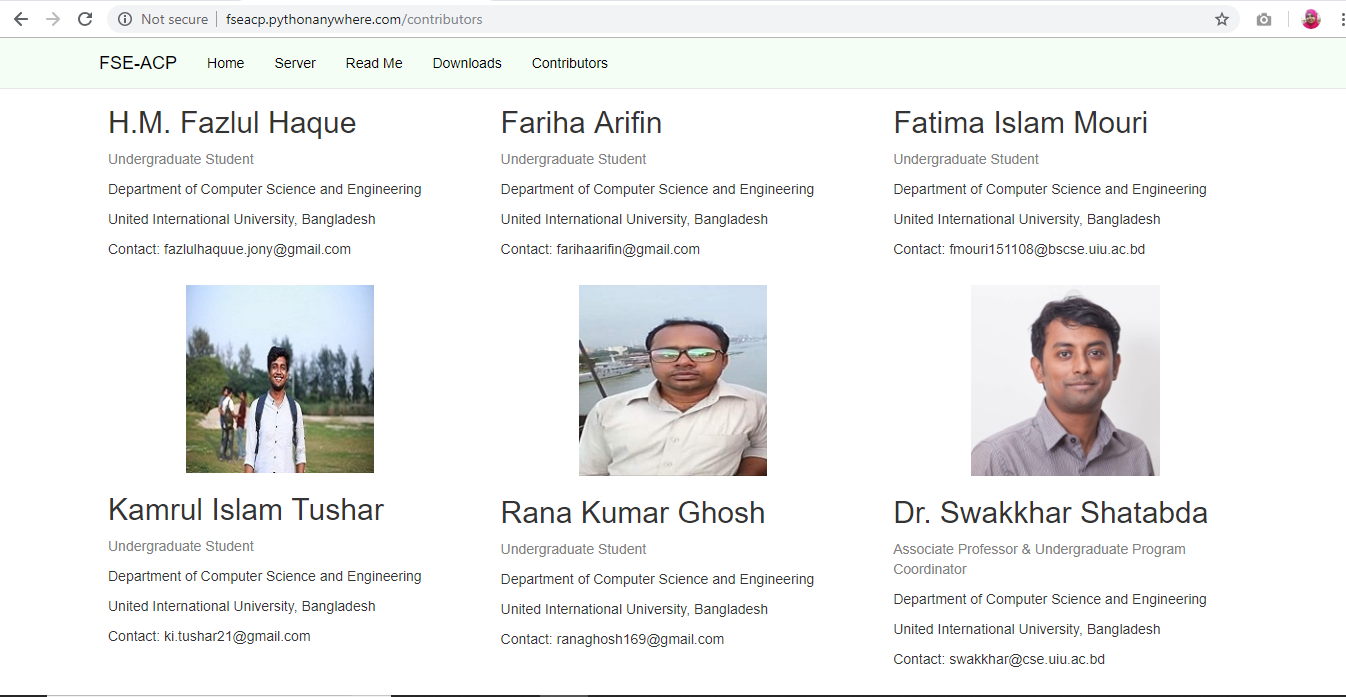
\includegraphics[width=0.8\textwidth]{contri2.png}
 \caption{Contributors Page}
\end{figure}
\begin{figure}[H]
\centering
 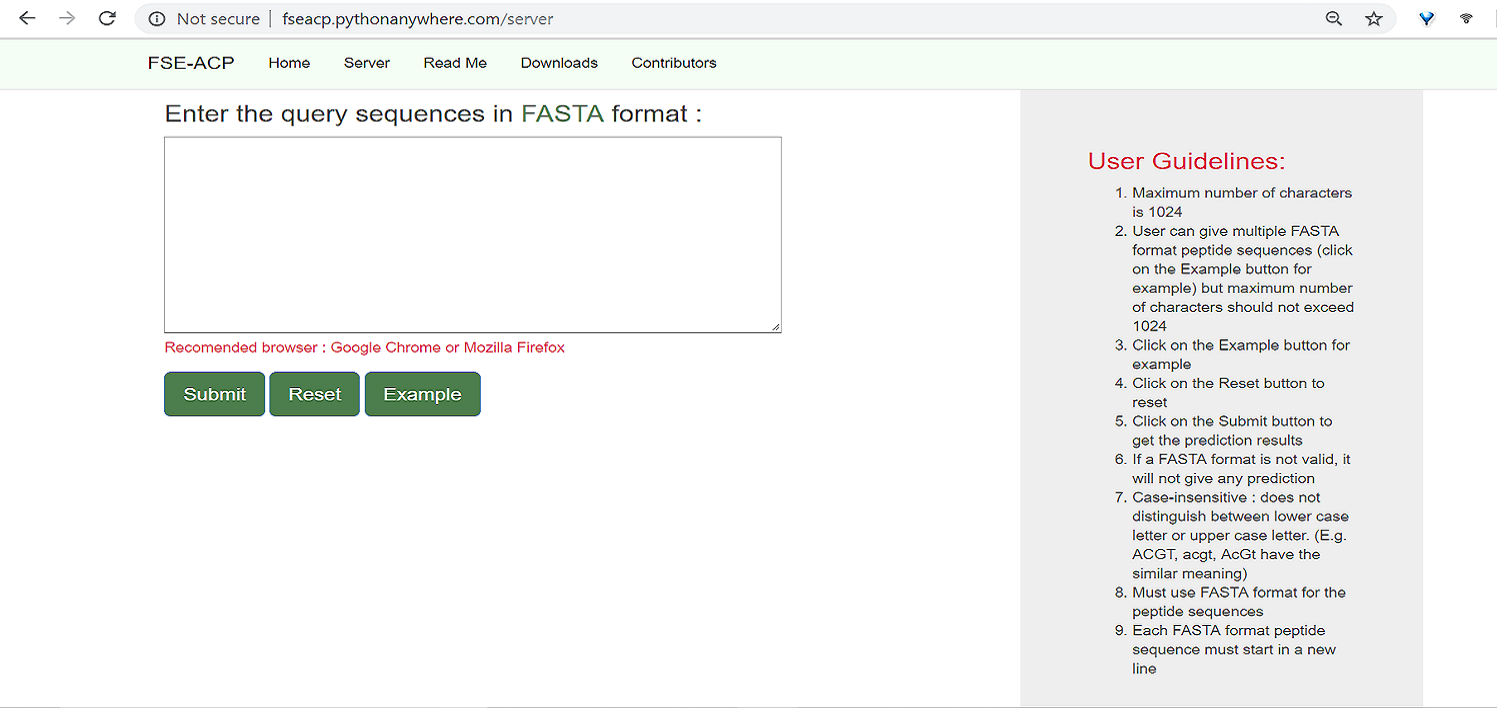
\includegraphics[width=0.8\textwidth]{server1.png}
 \caption{Server main Page}
\end{figure}
\begin{figure}[H]
\centering
 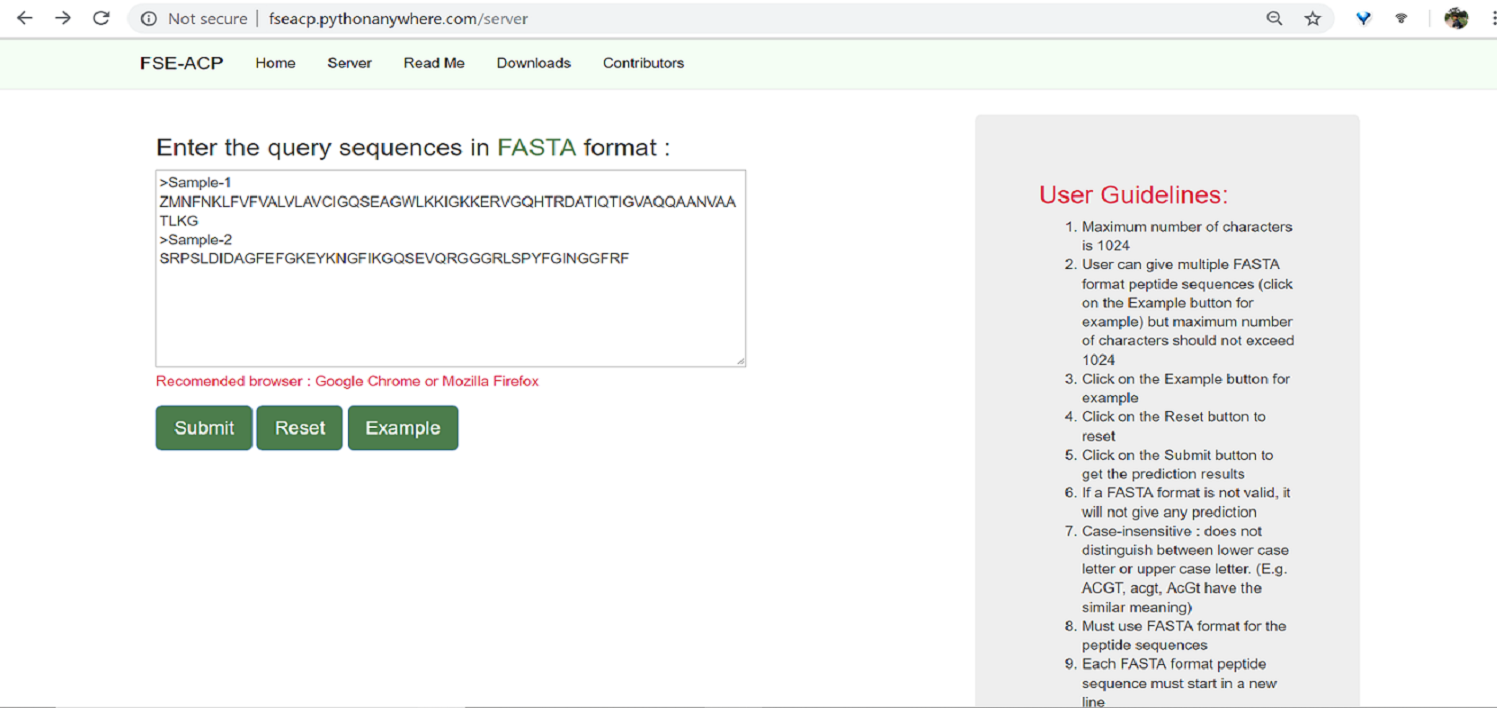
\includegraphics[width=0.8\textwidth]{server2.png}
 \caption{Server Page(with example data)}
\end{figure}
\begin{figure}[H]
\centering
 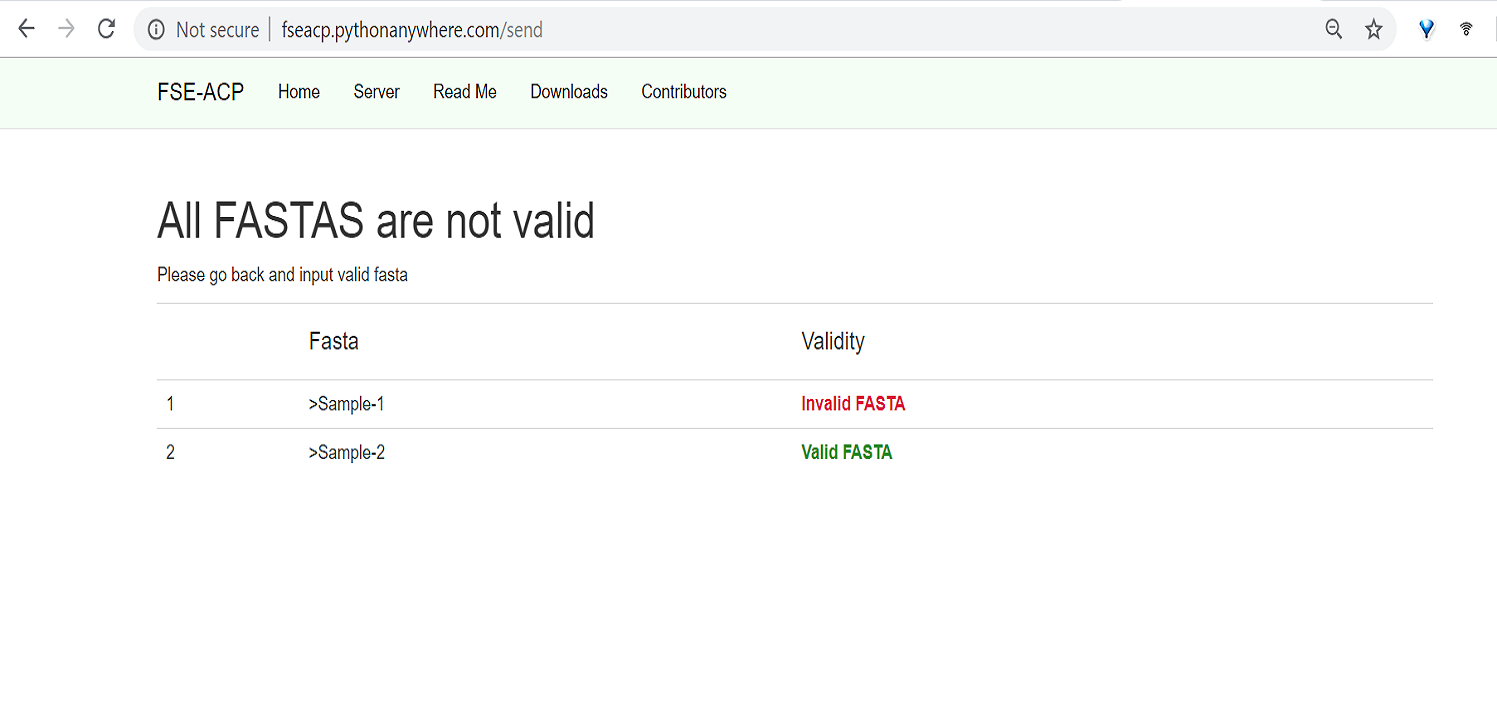
\includegraphics[width=0.8\textwidth]{server3.png}
 \caption{Server Page(result of example data)}
\end{figure}
\begin{figure}[H]
\centering
 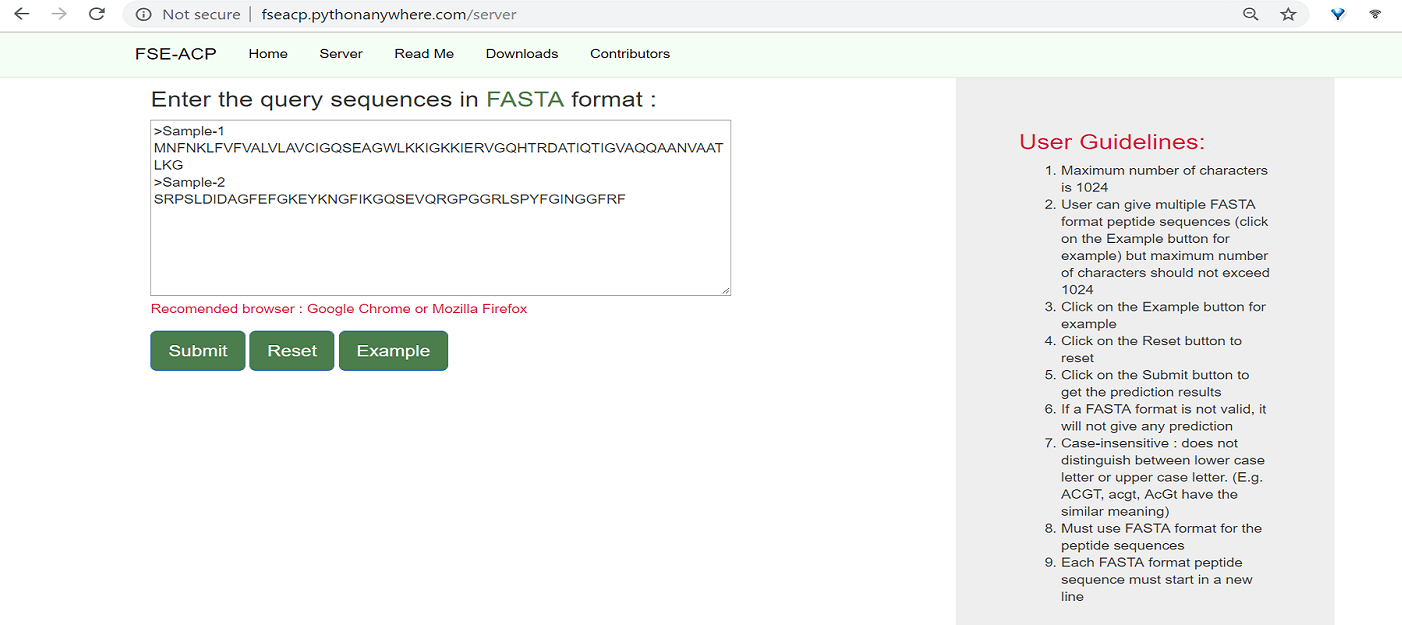
\includegraphics[width=0.8\textwidth]{server4.png}
 \caption{Server Page(with other data)}
\end{figure}
\begin{figure}[H]
\centering
 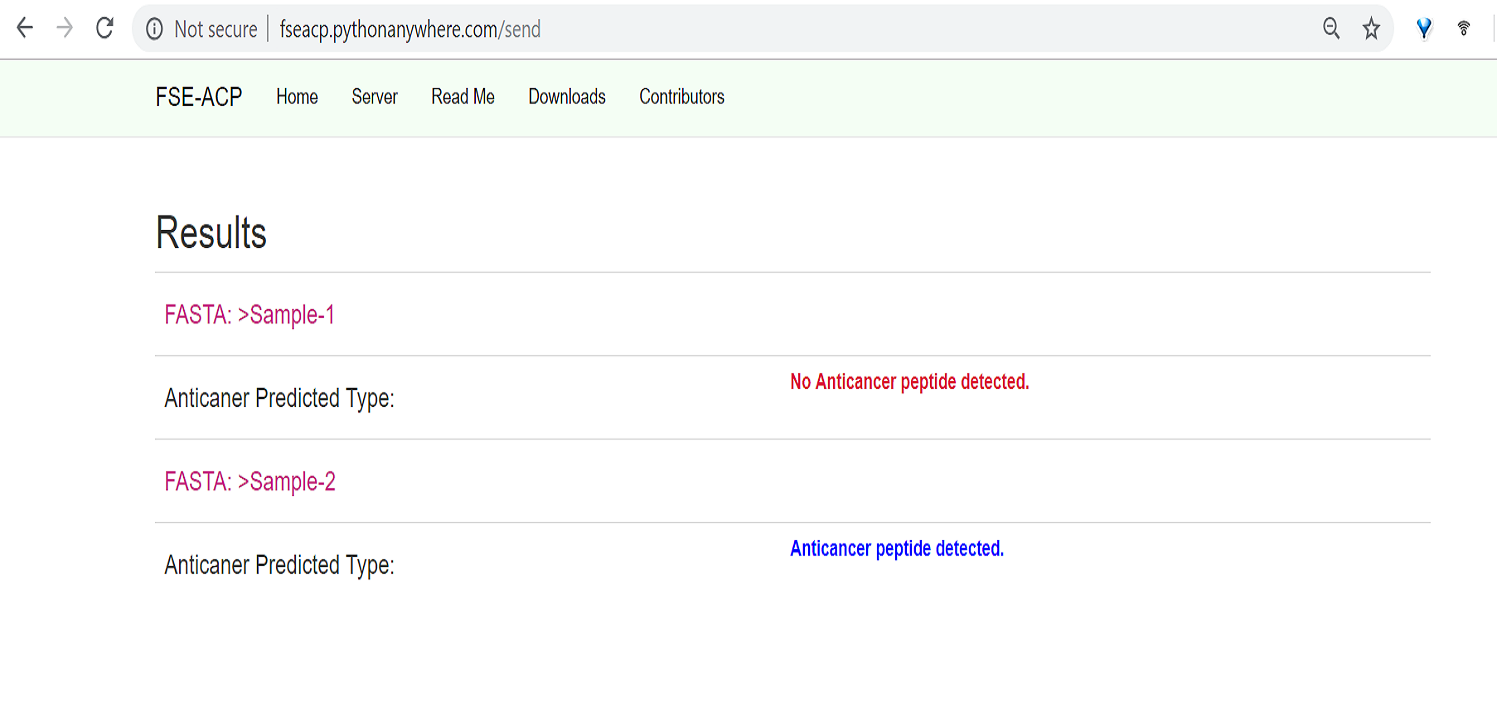
\includegraphics[width=0.8\textwidth]{server5.png}
 \caption{Server Page(result of other data)}
\end{figure}

\chapter{Conclusion} \label{Conclusion}

\ifpdf
    \graphicspath{{chapter_6/figures/PNG/}{chapter_6/figures/PDF/}{chapter_5/figures/}}
\else
    \graphicspath{{chapter_6/figures/EPS/}{chapter_6/figures/}}
\fi

\section{Summary}

In this project, we present a novel ensemble based classification method and a web base tool based on feature subspacing and apply it for solving anticancer peptide prediction problem. On the standard benchmark dataset, our method produces significantly better results compared to single weak classifiers and outperforms most other state-of-the-art predictors. However, there are still a room to improve in terms of accuracy. We believe, more effective feature space and feature selection might result into more effective classifier.

\section{Limitation}

We have time constraints, that we may need more time to more feature selection to achieve the higher accuracy we want but we have time limitation to finish the work. We are using free software so there is no constraint on that part. Even for using dataset we do not need to take any permission as it is open for anyone to use.

\section{Future Work}
In future we will apply feature selection to increase our present accuracy and try to apply our model on independent dataset. We will try to find more features and try to apply this subspacing method on various types of datasets. We will increase tool's usability and also try to publish it as a journal.





\bibliographystyle{6_backmatter/IEEEtran}

\bibliography{6_backmatter/Farid_bib} 

%% ----------------------------------------------------------------
% Now begin the Appendices, including them as separate files
\addtocontents{toc}{\vspace{2em}} % Add a gap in the Contents, for aesthetics
%\appendix % Cue to tell LaTeX that the following 'chapters' are Appendices
%% Appendix A
\chapter{Appendix Title}
\label{AppendixA}
\lhead{Appendix A. \emph{Data}}
\small

\section{Section Title}
Write section here.

\subsection{Sub-section here}
Write sub-section here.	% Appendix Title
%% Appendix B
\chapter{Appendix Title}
\label{AppendixB}
\lhead{Appendix B. \emph{Supervised Learning using na\"\i ve Bayesian Classifier}}
\ifpdf
    \graphicspath{{8_backmatter/figures/PNG/}{8_backmatter/figures/PDF/}{8_backmatter/figures/}}
\else
    \graphicspath{{8_backmatter/figures/EPS/}{8_backmatter/figures/}}
\fi

Add appendix here.


	
\addtocontents{toc}{\vspace{2em}}  % Add a gap in the Contents, for aesthetics
\backmatter
\end{document}
